\documentclass{report}
\usepackage{graphicx}
\usepackage[top=1in, bottom=1in, left=0.5in, right=0.5in]{geometry}
\usepackage{amsmath}
\usepackage{lscape}
\graphicspath{ {images/} }

\usepackage{biblatex}
\bibliography{../books}
\title{Amplifier Topologies}
\author{Simon Hobbs}
\newcommand{\imwidth}{0.2\textwidth}

\begin{document}
\maketitle

\chapter{Amplifiers}

\section{Functional Types}
\label{sec:ampTypes}
\begin{table}[h!]
    \caption{Types of amplifiers by function}
\begin{description}
    \item[Voltage]
        Voltage in, voltage out. Need high impedance in, low out.
    \item[Current]
        Current in, current out. Need low impedance in, high out.
    \item[Transimpedance]
        Current in, voltage out. Need low impedance in, low out.
    \item[Transconductance]
        Voltage in, current out. Need high impedance in, high out.
\end{description}
\end{table}
For a voltage input you want high impedance so that the signal is not loaded and therefore distorted by the amp regardless of the
impedance of the source.
For voltage output you want low impedance so that the signal is not distorted by the load.
For current input you want low impedance so that the source can drive the signal without the current being distorted.
For current output you want high impedance as a high output impedance reduces the effect of a finite resistance in the 
current source, the higher the ratio of Z$_{load}$/Z$_{intrinsic}$ the closer to ideal the amp.

Combining different section of these basic types can better address the design goals than just one.
A transconductance amp cannot drive a large load without significant distortion, so a current amp following would
allow a load to be driven without distortion.

\section{Choosing BJTs or FETs}
\subsection{BJT Issues}
\begin{description}
    \item[Miller Effect]
    \item[Early Voltage]
    \item[Thermal Runaway]
    \item[Base Current]
    \item[Temperature Drift]
\end{description}

\subsection{JFET Issues}
\begin{description}
    \item[Component Variability]
    \item[Low Gain]
    \item[Noise]
\end{description}

\chapter{OPAMPS}
\section{When Not to use an OPAMP}
\section{Flaws}
\subsection{Slew Rate}
\subsection{Noise}
\subsection{Saturation}
\subsection{Common Mode Gain}
\subsection{Power Supply Rejection}
\subsection{Temperature Drift}
\subsection{Input Capacitance}


\chapter{Basic Single BJT}
\section{Analysis Techniques}
\subsection{$\beta$ Transform}
Assume that the transistor is in the active region, take the definition of $\beta$:
\begin{equation}
    \label{eqn:beta}
    i_{e} \equiv (\beta + 1) \cdot i_{b}
\end{equation}
to move the resistor terms from the base to the emitter or from the emitter to the base (whichever is more convenient).
The you can calculate the gain etc. using Kirkoffs laws.

\section{Common-Emitter}
\begin{figure}
\centering
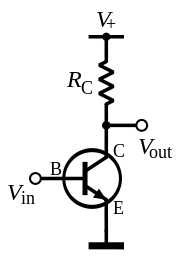
\includegraphics[width = \imwidth]{NPN_common_emitter}
\caption{}
\end{figure}

\section{Common-Base}
\begin{figure}
\centering
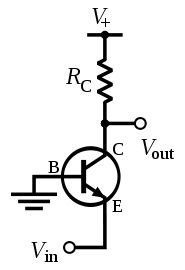
\includegraphics[width = \imwidth]{NPN_common_base}
\caption{}
\end{figure}

\section{Common-Collector}
AKA emitter follower
\begin{figure}
\centering
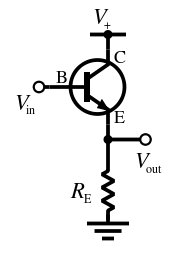
\includegraphics[width = \imwidth]{NPN_common_collector}
\caption{}
\end{figure}

\section{Comparison}
The three single BJT amplifier types have different applications for the different amplifier types (Section \ref{sec:ampTypes}).
\begin{table}
    \centering
    \caption{Comparison of the three basic BJT amps}
    \begin{tabular}{llll}
        \hline\hline
        \textbf{Type} &\textbf{Input Impedance}&\textbf{Ouput Impedance}&\textbf{Ideal Amp Use}\\\hline
        CC & Large & Medium& Voltage\\
        CB & Small & Medium& TIA\\
        CE & Large & Small & Voltage, Current, TCA\\
        \hline\hline
    \end{tabular}
\end{table}

\chapter{Basic Single FET}
\section{Common-Source}
\section{Common-Gate}
\section{Common-Drain}

\chapter{Multisection BJT Amps}
\section{Cascade}
\begin{figure}
\centering
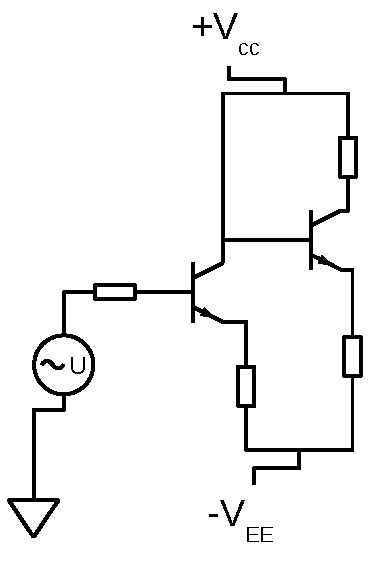
\includegraphics[width = \imwidth]{cascade}
\caption{}
\end{figure}


\section{Cascode}
\begin{figure}
\centering
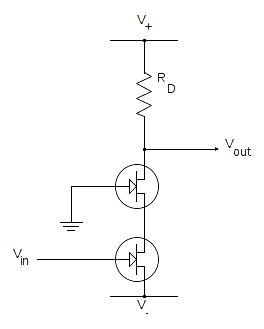
\includegraphics[width = \imwidth]{CascodeWithNegative}
\caption{}
\end{figure}


\section{Darlington}
Basically a super $\beta$, slow BJT.

\section{Differential Emitter-Coupled}
AKA Long-tail
\begin{figure}
\centering
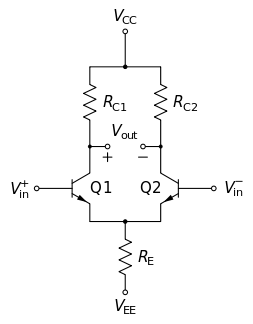
\includegraphics[width = \imwidth]{Differential_amplifier_long-tailed_pair}
\caption{}
\end{figure}


\section{Current Mirrors}
\begin{figure}
\centering
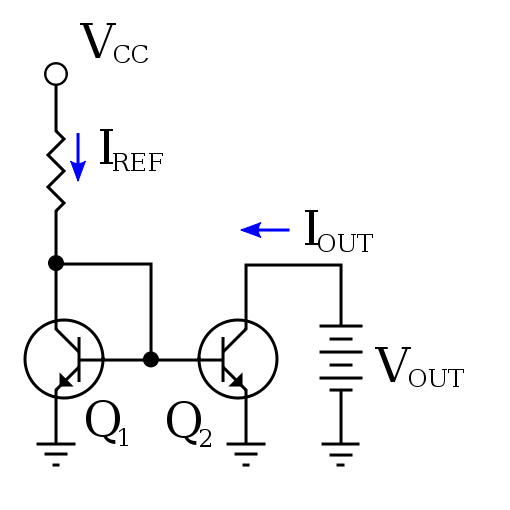
\includegraphics[width = \imwidth]{Simple_bipolar_mirror}
\caption{}
\end{figure}


\chapter{Amplifier Concepts}
\section{Emitter Degeneration}
\section{Bootstraping}

\nocite{*}
\printbibliography
\end{document}
